\chapter*{Installation}
\label{cha:installation}

\section{Choix}
\label{sec:choix}

\subsection{Distribution}
\label{sec:distribution}

Notre choix de la distribution s'est naturellement porté sur Debian, pour ses
nombreux avantages. En voici quelques exemples :

\begin{itemize}
\item Large communauté : grâce à cela, les erreurs et problèmes rencontrés ont
  souvent plusieurs solutions connues et éprouvées.

\item Plusieurs architectures et noyaux : Debian supporte la majorité des
  architectures de processeurs comme AMD, Armel, i386, MIPS, etc. Elle supporte
  aussi de nombreux noyaux tels que FreeBSD et GNU Hurd.

\item Sécurité : vu que la distribution est open-source, cela signifie que les
  backdoors sont presque inexistantes. De surcroît, lorsqu'une faille de sécurité
  est détectée, celle-ci est rapidement corrigée par la communauté.

  En outre, Debian comprend de nombreux logiciels de sécurité tels que GPG (et
  PGP), SSH et autres.

\item Stabilité : nous savons que les serveurs doivent avoir le plus grand temps
d'accessibilité ($\approx$ 99.999\%). Sous Debian, il existe de nombreux exemples de
machines qui tournent sans arrêt pendant des années, mis à part lors de pannes
ou de mises à jour matérielles.

\item Système de paquets : grâce au système de paquets, les distributions Linux
ont la possibilité d'installer de nombreux logiciels par une seule ligne de
commande. Le système de paquets de Debian est l'outil central de mise à jour,
installation, suppression et recherche de paquets.
\end{itemize}

\newpage

De même, la distribution Debian est plus professionnel et celle-ci possède le
leadership depuis des années.

À titre d'information, depuis mai 2016, Ubuntu a les mêmes parts de marché que
Debian.

\begin{figure}[!h]
    \center
    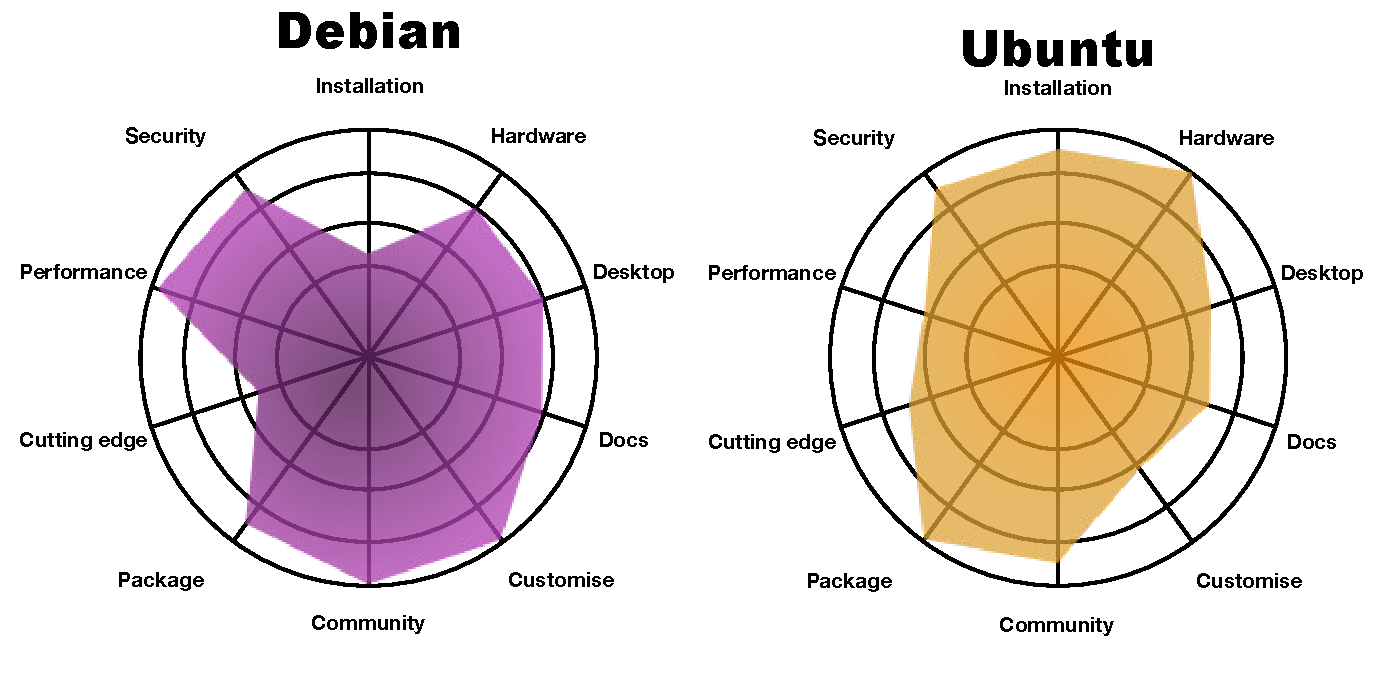
\includegraphics[scale=0.35]
    {textures/images/installation/DebianVsUbuntu.pdf}
    \caption{Différences entre Debian et Ubuntu}
  \end{figure}

Nous n'avons pas choisi Ubuntu pour les raisons suivantes :

\begin{itemize}
\item C'est un dérivé de Debian : de ce fait, un administrateur sachant
  configurer un serveur Debian pourra faciliter s'adapter au serveur Ubuntu.

\item Il vise le grand public et, de ce fait, est beaucoup moins utilisé
  dans le milieu professionnel.

\item Celui-ci est assez récent sur le marché du serveur.

\item Moins performant que Debian.
\end{itemize}

Concernant les autres distributions, CentOS est en baisse, mais reste au-dessus
de Red Hat et de Fedora qui, lui, est en chute libre.

\begin{figure}[h]
  \centering
  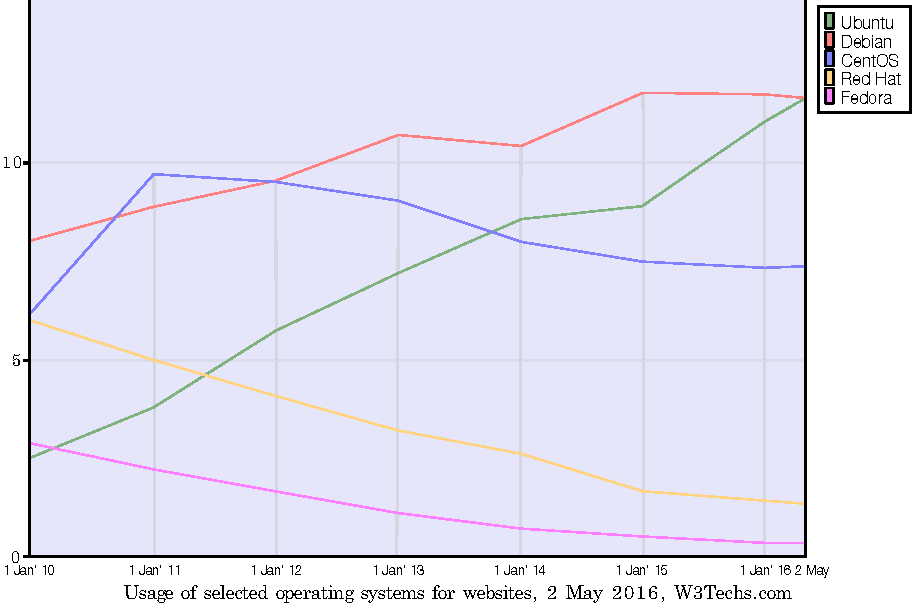
\includegraphics[scale=0.65]
  {textures/images/installation/distributions.pdf}
  \caption{Parts de marché des distributions Linux}
\end{figure}

\newpage

\subsection{Langue}
\label{sec:langue}

Pour le choix de la langue lors de l'installation, il a été préféré d'utiliser
l'anglais vu que la majorité des documentations et forums sont disponibles dans
cette langue. De plus, cela permet d'éviter une mauvaise traduction concernant
les nouvelles mises à jour et de toucher un plus large public possible.

\subsection{Noyau}
\label{sec:noyau}

Un noyau (monolithique) modulaire a été choisi afin de gérer les
modules. En effet, celui-ci facilite l'ajout et la suppression de modules à
chaud. Ces modules, pas toujours indispensables, peuvent être la source de
failles et de bugs.

%%% Local Variables:
%%% mode: latex
%%% TeX-master: t
%%% End:
